\PassOptionsToPackage{unicode=true}{hyperref} % options for packages loaded elsewhere
\PassOptionsToPackage{hyphens}{url}
%
\documentclass[]{article}
\usepackage{lmodern}
\usepackage{amssymb,amsmath}
\usepackage{ifxetex,ifluatex}
\usepackage{fixltx2e} % provides \textsubscript
\ifnum 0\ifxetex 1\fi\ifluatex 1\fi=0 % if pdftex
  \usepackage[T1]{fontenc}
  \usepackage[utf8]{inputenc}
  \usepackage{textcomp} % provides euro and other symbols
\else % if luatex or xelatex
  \usepackage{unicode-math}
  \defaultfontfeatures{Ligatures=TeX,Scale=MatchLowercase}
    \setmainfont[]{Arial}
\fi
% use upquote if available, for straight quotes in verbatim environments
\IfFileExists{upquote.sty}{\usepackage{upquote}}{}
% use microtype if available
\IfFileExists{microtype.sty}{%
\usepackage[]{microtype}
\UseMicrotypeSet[protrusion]{basicmath} % disable protrusion for tt fonts
}{}
\IfFileExists{parskip.sty}{%
\usepackage{parskip}
}{% else
\setlength{\parindent}{0pt}
\setlength{\parskip}{6pt plus 2pt minus 1pt}
}
\usepackage{hyperref}
\hypersetup{
            pdftitle={Problem Set 02: Data Visualization},
            pdfborder={0 0 0},
            breaklinks=true}
\urlstyle{same}  % don't use monospace font for urls
\usepackage[margin=1in]{geometry}
\usepackage{color}
\usepackage{fancyvrb}
\newcommand{\VerbBar}{|}
\newcommand{\VERB}{\Verb[commandchars=\\\{\}]}
\DefineVerbatimEnvironment{Highlighting}{Verbatim}{commandchars=\\\{\}}
% Add ',fontsize=\small' for more characters per line
\usepackage{framed}
\definecolor{shadecolor}{RGB}{248,248,248}
\newenvironment{Shaded}{\begin{snugshade}}{\end{snugshade}}
\newcommand{\AlertTok}[1]{\textcolor[rgb]{0.94,0.16,0.16}{#1}}
\newcommand{\AnnotationTok}[1]{\textcolor[rgb]{0.56,0.35,0.01}{\textbf{\textit{#1}}}}
\newcommand{\AttributeTok}[1]{\textcolor[rgb]{0.77,0.63,0.00}{#1}}
\newcommand{\BaseNTok}[1]{\textcolor[rgb]{0.00,0.00,0.81}{#1}}
\newcommand{\BuiltInTok}[1]{#1}
\newcommand{\CharTok}[1]{\textcolor[rgb]{0.31,0.60,0.02}{#1}}
\newcommand{\CommentTok}[1]{\textcolor[rgb]{0.56,0.35,0.01}{\textit{#1}}}
\newcommand{\CommentVarTok}[1]{\textcolor[rgb]{0.56,0.35,0.01}{\textbf{\textit{#1}}}}
\newcommand{\ConstantTok}[1]{\textcolor[rgb]{0.00,0.00,0.00}{#1}}
\newcommand{\ControlFlowTok}[1]{\textcolor[rgb]{0.13,0.29,0.53}{\textbf{#1}}}
\newcommand{\DataTypeTok}[1]{\textcolor[rgb]{0.13,0.29,0.53}{#1}}
\newcommand{\DecValTok}[1]{\textcolor[rgb]{0.00,0.00,0.81}{#1}}
\newcommand{\DocumentationTok}[1]{\textcolor[rgb]{0.56,0.35,0.01}{\textbf{\textit{#1}}}}
\newcommand{\ErrorTok}[1]{\textcolor[rgb]{0.64,0.00,0.00}{\textbf{#1}}}
\newcommand{\ExtensionTok}[1]{#1}
\newcommand{\FloatTok}[1]{\textcolor[rgb]{0.00,0.00,0.81}{#1}}
\newcommand{\FunctionTok}[1]{\textcolor[rgb]{0.00,0.00,0.00}{#1}}
\newcommand{\ImportTok}[1]{#1}
\newcommand{\InformationTok}[1]{\textcolor[rgb]{0.56,0.35,0.01}{\textbf{\textit{#1}}}}
\newcommand{\KeywordTok}[1]{\textcolor[rgb]{0.13,0.29,0.53}{\textbf{#1}}}
\newcommand{\NormalTok}[1]{#1}
\newcommand{\OperatorTok}[1]{\textcolor[rgb]{0.81,0.36,0.00}{\textbf{#1}}}
\newcommand{\OtherTok}[1]{\textcolor[rgb]{0.56,0.35,0.01}{#1}}
\newcommand{\PreprocessorTok}[1]{\textcolor[rgb]{0.56,0.35,0.01}{\textit{#1}}}
\newcommand{\RegionMarkerTok}[1]{#1}
\newcommand{\SpecialCharTok}[1]{\textcolor[rgb]{0.00,0.00,0.00}{#1}}
\newcommand{\SpecialStringTok}[1]{\textcolor[rgb]{0.31,0.60,0.02}{#1}}
\newcommand{\StringTok}[1]{\textcolor[rgb]{0.31,0.60,0.02}{#1}}
\newcommand{\VariableTok}[1]{\textcolor[rgb]{0.00,0.00,0.00}{#1}}
\newcommand{\VerbatimStringTok}[1]{\textcolor[rgb]{0.31,0.60,0.02}{#1}}
\newcommand{\WarningTok}[1]{\textcolor[rgb]{0.56,0.35,0.01}{\textbf{\textit{#1}}}}
\usepackage{graphicx,grffile}
\makeatletter
\def\maxwidth{\ifdim\Gin@nat@width>\linewidth\linewidth\else\Gin@nat@width\fi}
\def\maxheight{\ifdim\Gin@nat@height>\textheight\textheight\else\Gin@nat@height\fi}
\makeatother
% Scale images if necessary, so that they will not overflow the page
% margins by default, and it is still possible to overwrite the defaults
% using explicit options in \includegraphics[width, height, ...]{}
\setkeys{Gin}{width=\maxwidth,height=\maxheight,keepaspectratio}
\setlength{\emergencystretch}{3em}  % prevent overfull lines
\providecommand{\tightlist}{%
  \setlength{\itemsep}{0pt}\setlength{\parskip}{0pt}}
\setcounter{secnumdepth}{0}
% Redefines (sub)paragraphs to behave more like sections
\ifx\paragraph\undefined\else
\let\oldparagraph\paragraph
\renewcommand{\paragraph}[1]{\oldparagraph{#1}\mbox{}}
\fi
\ifx\subparagraph\undefined\else
\let\oldsubparagraph\subparagraph
\renewcommand{\subparagraph}[1]{\oldsubparagraph{#1}\mbox{}}
\fi

% set default figure placement to htbp
\makeatletter
\def\fps@figure{htbp}
\makeatother


\title{Problem Set 02: Data Visualization}
\author{}
\date{\vspace{-2.5em}}

\begin{document}
\maketitle

{
\setcounter{tocdepth}{2}
\tableofcontents
}
In this problem set we will use the \texttt{ggplot2} package to generate
graphics. The ``The Grammar of Graphics'' is the theoretical basis for
the \texttt{ggplot2} package. Much like how we construct sentences in
any language by using a linguistic grammar (nouns, verbs, etc.), the
grammar of graphics allows us to specify the components of a statistical
graphic.

In short, the grammar tells us that:

\begin{quote}
A statistical graphic is a \texttt{mapping} of \texttt{data} variables
to \texttt{aes}thetic attributes of \texttt{geom}etric objects.
\end{quote}

We can break a graphic into the following three \textbf{essential}
components:

\begin{itemize}
\tightlist
\item
  \texttt{data}: the data-set comprised of variables that we plot
\item
  \texttt{geom}: this refers to our type of \texttt{geom}etric objects
  we see in our plot (points, lines, bars, etc.)
\item
  \texttt{aes}: aesthetic attributes of the geometric object that we can
  perceive on a graphic. For example, x/y position, color, shape, and
  size. Each assigned aesthetic attribute can be mapped to a variable in
  our data-set.
\end{itemize}

\hypertarget{getting-set-up}{%
\section{Getting Set up}\label{getting-set-up}}

Go ahead and launch RStudio, and open a new R Markdown file. Recall, to
open a new R Markdown (.Rmd) file:

\begin{itemize}
\tightlist
\item
  Click on the little green plus on the upper left of the window.
\item
  Select R Markdown, as in the image below.
\end{itemize}

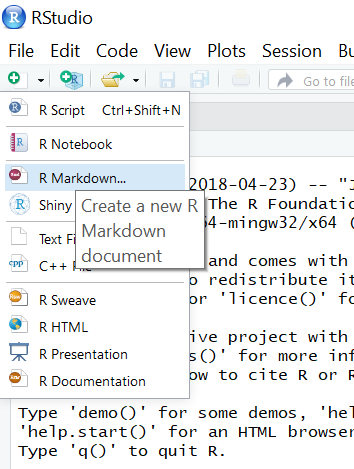
\includegraphics[width=2.08333in,height=\textheight]{figures/how.to.open.rmd.png}

Once you have opened the document:

\begin{itemize}
\tightlist
\item
  Change the title at the top to ``Data Visualisation''. Be sure to keep
  the quotation marks.
\item
  Add an author line, following the example below. You need quotation
  marks!
\item
  Delete any extra code (everything from line 7 down).
\end{itemize}

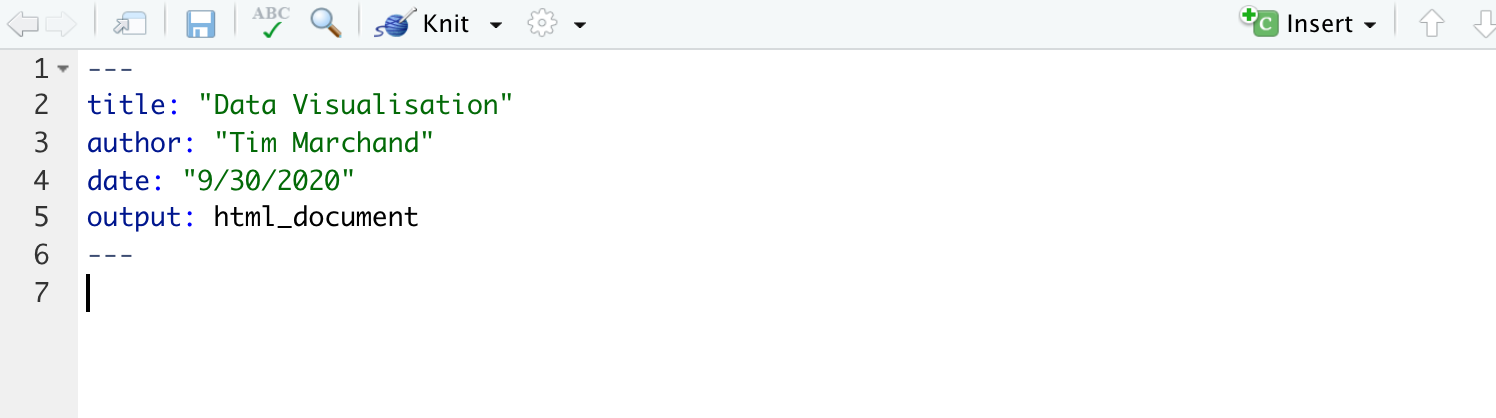
\includegraphics[width=1\textwidth,height=\textheight]{figures/set_up.png}

Finally, save your new R Markdown document:

\begin{itemize}
\tightlist
\item
  Click File \textgreater{} Save As\ldots{}
\item
  Browse to the folder where you want to store the R Markdown document
  and its output.
\item
  Name the file something informative, e.g.,
  \texttt{PS02\_lastname\_firstname} (fill in your first name and last
  name). Make sure to keep the \texttt{.Rmd} file extension.
\end{itemize}

You will hand in a \textbf{knitted pdf file} as your problem set. It is
OK if your lab report includes the example code from the lab, as well as
your Exercises. Just be sure to \textbf{make a header to label each
Exercise}. Please type your code to answer the questions in a code chunk
(gray part), under the exercise headers and type (\textbf{BRIEF})
answers to any interpretation questions in the white part under the
headers.

\hypertarget{r-packages}{%
\subsubsection{R Packages}\label{r-packages}}

For this problem set we will use the following R packages:

\begin{itemize}
\tightlist
\item
  \texttt{dplyr}: for data wrangling
\item
  \texttt{ggplot2}: for data visualization
\item
  \texttt{readr}: for reading in data
\end{itemize}

Copy, paste and run the following in a code chunk (see the figure above
if you forget how to insert a code chunk).

\begin{Shaded}
\begin{Highlighting}[]
\KeywordTok{library}\NormalTok{(dplyr)}
\KeywordTok{library}\NormalTok{(ggplot2)}
\KeywordTok{library}\NormalTok{(readr)}
\end{Highlighting}
\end{Shaded}

Remember, ``running code means'' telling R ``do this''. You tell R to do
something by passing it through the console. You can run existing code
many ways:

\begin{itemize}
\tightlist
\item
  Re-typing code out directly in the console (most laborious method)
\item
  Copying and pasting existing code into the console and hitting enter
  (easier method)
\item
  Click on the green triangle in the code chunk (easiest method 1)
\item
  Highlight the code and hit \texttt{Control-Enter} on PC or
  \texttt{Command-Return} on a Mac (easiest method 2).
\end{itemize}

\hypertarget{the-data}{%
\subsubsection{The Data}\label{the-data}}

Today we will practice data visualization using data on births from the
state of North Carolina. Copy, paste and run the code below to load the
data.

\begin{Shaded}
\begin{Highlighting}[]
\NormalTok{nc <-}\StringTok{ }\KeywordTok{read_csv}\NormalTok{(}\StringTok{"https://docs.google.com/spreadsheets/d/e/2PACX-1vTm2WZwNBoQdZhMgot7urbtu8eG7tzAq-60ZJsQ_nupykCAcW0OXebVpHksPWyR4x8xJTVQ8KAulAFS/pub?gid=202410847&single=true&output=csv"}\NormalTok{)}
\end{Highlighting}
\end{Shaded}

The workspace area in the upper right hand corner of the R Studio window
should now list a data set called \texttt{nc} with 800 observations
(rows or cases) and 13 variables (columns). Each observation or
\textbf{case} is a birth of a single child.

\hypertarget{how-to-look-at-data-in-r}{%
\section{How to look at data in R}\label{how-to-look-at-data-in-r}}

\hypertarget{take-a-glimpse}{%
\subsubsection{Take a glimpse}\label{take-a-glimpse}}

You can see the \textbf{dimensions of this data frame (\# of rows and
columns)}, the names of the variables, the variable types, and the first
few observations using the \texttt{glimpse} function. Copy, paste, and
run the following in a new code chunk.

\begin{Shaded}
\begin{Highlighting}[]
\KeywordTok{glimpse}\NormalTok{(nc)}
\end{Highlighting}
\end{Shaded}

We can see that there are 1000 observations and 13 variables in this
data set. The variable names are \texttt{fage}, \texttt{mage},
\texttt{mature}, etc. This output also tells us that some variables are
numbers\ldots{}some specifically integers
\texttt{\textless{}int\textgreater{}}, others are numbers with decimals
\texttt{\textless{}dbl\textgreater{}}. Some of the variables are factors
\texttt{\textless{}fct\textgreater{}}. It is a good practice to see if R
is treating variables as factors \texttt{\textless{}fct\textgreater{}};
as numbers \texttt{\textless{}int\textgreater{}} or
\texttt{\textless{}dbl\textgreater{}} (basically numbers with decimals);
or as characters (i.e.~text) \texttt{\textless{}chr\textgreater{}}.

\begin{enumerate}
\def\labelenumi{\arabic{enumi}.}
\tightlist
\item
  What type of variable is R considering the variable \texttt{habit} to
  be? What variable type is \texttt{visits}? (Answer with text)
\end{enumerate}

\hypertarget{the-data-viewer}{%
\subsubsection{The data viewer}\label{the-data-viewer}}

You can view the data by clicking on the name \texttt{nc} in the
\emph{Environment} pane (upper right window). This will bring up an
alternative display of the data set in the \emph{Data Viewer} (upper
left window). R has stored these data in a kind of spreadsheet called a
\emph{data frame}. Each row represents a different birth: the first
entry or column in each row is simply the row number, the rest are the
different variables that were recorded for each birth. You can close the
data viewer by clicking on the \texttt{x} in the upper left hand corner.

\leavevmode\hypertarget{license}{}%
It is a good idea to try kitting your document from time to time as you
go along! Go ahead, and make sure your document is knitting, and that
your knitted file includes Exercise headers, text, and code. Note that
knitting automatically saves your Rmd file too!

\hypertarget{types-of-graphs}{%
\section{Types of Graphs}\label{types-of-graphs}}

We will explore three different types of graphs in this problem set.

\begin{itemize}
\tightlist
\item
  Scatterplots
\item
  Boxplots
\item
  Histograms
\end{itemize}

\hypertarget{scatterplots}{%
\subsection{Scatterplots}\label{scatterplots}}

Scatterplots allow you to investigate the relationship between two
\textbf{numerical} variables. While you may already be familiar with
this type of plot, let's view it through the lens of the Grammar of
Graphics. Specifically, we will graphically investigate the relationship
between the following two numerical variables in the \texttt{nc} data
frame:

\begin{itemize}
\tightlist
\item
  \texttt{weeks}: length of a pregnancy on the horizontal ``x'' axis and
\item
  \texttt{weight}: birth weight of a baby in pounds on the vertical
  ``y'' axis
\end{itemize}

\begin{Shaded}
\begin{Highlighting}[]
\KeywordTok{ggplot}\NormalTok{(}\DataTypeTok{data =}\NormalTok{ nc, }\KeywordTok{aes}\NormalTok{(}\DataTypeTok{x =}\NormalTok{ weeks, }\DataTypeTok{y =}\NormalTok{ weight)) }\OperatorTok{+}\StringTok{ }
\StringTok{  }\KeywordTok{geom_point}\NormalTok{()}
\end{Highlighting}
\end{Shaded}

\includegraphics{PS02_data_viz_files/figure-latex/unnamed-chunk-5-1.pdf}

Let's view this plot through the grammar of graphics. Within the
\texttt{ggplot()} function call, we specified:

\begin{itemize}
\tightlist
\item
  The data frame to be \texttt{nc} by setting \texttt{data\ =\ nc}
\item
  The \texttt{aes}thetic \texttt{mapping} by setting
  \texttt{aes(x\ =\ weeks,\ y\ =\ weight)}
\item
  The variable \texttt{weeks} maps to the \texttt{x}-position
  \texttt{aes}thetic
\item
  The variable \texttt{weight} maps to the \texttt{y}-position
  \texttt{aes}thetic.
\end{itemize}

We also add a layer to the \texttt{ggplot()} function call using the
\texttt{+} sign. The layer in question specifies the \texttt{geom}etric
object here as \texttt{point}s, by specifying \texttt{geom\_point()}.

Finally, we can also add axis labels and a title to the plot like so.
Again we add a new layer, this time a \texttt{labs} or labels layer.

\begin{Shaded}
\begin{Highlighting}[]
\KeywordTok{ggplot}\NormalTok{(}\DataTypeTok{data =}\NormalTok{ nc, }\KeywordTok{aes}\NormalTok{(}\DataTypeTok{x =}\NormalTok{ weeks, }\DataTypeTok{y =}\NormalTok{ weight)) }\OperatorTok{+}\StringTok{ }
\StringTok{  }\KeywordTok{geom_point}\NormalTok{() }\OperatorTok{+}\StringTok{ }
\StringTok{  }\KeywordTok{labs}\NormalTok{(}\DataTypeTok{x =} \StringTok{"Length of pregnancy (in weeks)"}\NormalTok{, }\DataTypeTok{y =} \StringTok{"Birth weight of baby (lbs)"}\NormalTok{, }
       \DataTypeTok{title =} \StringTok{"Relationship between pregnancy duration and newborn weight"}\NormalTok{)}
\end{Highlighting}
\end{Shaded}

\begin{enumerate}
\def\labelenumi{\arabic{enumi}.}
\item
  Is there a positive or negative relationship between these variables?
  (Text only to answer)
\item
  Make a graph showing \texttt{weeks} again on the x axis and the
  variable \texttt{gained} on the y axis (the amount of weight a mother
  gained during pregnancy). Include axis labels with measurement units,
  and a title. (R code only to answer)
\item
  Study the code below, and the resulting graphical output. Note that I
  added a new argument of \texttt{color\ =\ premie} \textbf{inside} the
  \texttt{aes}thetic mapping. The variable \texttt{premie} indicates
  whether a birth was early (premie) or went full term. Please answer
  with text:

  \textbf{A.} What did adding the argument \texttt{color\ =\ premie}
  accomplish?

  \textbf{B.} How many \textbf{variables} are now displayed on this
  plot?

  \textbf{C.} What appears to (roughly) be the pregnancy length cutoff
  for classifying a newborn as a ``premie''" versus a ``full term''.
\end{enumerate}

\begin{Shaded}
\begin{Highlighting}[]
\KeywordTok{ggplot}\NormalTok{(}\DataTypeTok{data =}\NormalTok{ nc, }\KeywordTok{aes}\NormalTok{(}\DataTypeTok{x =}\NormalTok{ weeks, }\DataTypeTok{y =}\NormalTok{ gained, }\DataTypeTok{color =}\NormalTok{ premie))}\OperatorTok{+}\StringTok{ }
\StringTok{  }\KeywordTok{geom_point}\NormalTok{() }\OperatorTok{+}\StringTok{ }
\StringTok{  }\KeywordTok{labs}\NormalTok{(}\DataTypeTok{x =} \StringTok{"Pregnancy length (wks)"}\NormalTok{, }\DataTypeTok{y =} \StringTok{"Maternal weight gain (lbs)"}\NormalTok{)}
\end{Highlighting}
\end{Shaded}

\includegraphics{PS02_data_viz_files/figure-latex/unnamed-chunk-8-1.pdf}

\begin{enumerate}
\def\labelenumi{\arabic{enumi}.}
\tightlist
\item
  Make a new scatterplot that shows a mothers age on the x axis
  (variable called \texttt{mage}) and birth weight of newborns on the y
  axis (\texttt{weight}). Color the points on the plot based on the
  gender of the resulting baby (variable called \texttt{gender}). Does
  there appear to be any strong relationship between a mother's age and
  the weight of her newborn? (R code and text to answer)
\end{enumerate}

\leavevmode\hypertarget{license}{}%
Make sure your document is knitting, and that your knitted file includes
Exercise headers, text, and code. Note that knitting automatically saves
your Rmd file too!

\hypertarget{histograms}{%
\subsection{Histograms}\label{histograms}}

Histograms are useful plots for showing how many elements of a
\textbf{single numerical} variable fall in specified bins. This is a
very useful way to get a sense of the \textbf{distribution} of your
data. Histograms are often one of the first steps in exploring data
visually.

For instance, to look at the distribution of pregnancy duration
(variable called \texttt{weeks}), copy, paste and run the following in a
new code chunk:

\begin{Shaded}
\begin{Highlighting}[]
\KeywordTok{ggplot}\NormalTok{(}\DataTypeTok{data =}\NormalTok{ nc, }\KeywordTok{aes}\NormalTok{(}\DataTypeTok{x =}\NormalTok{ weeks))}\OperatorTok{+}\StringTok{ }
\StringTok{  }\KeywordTok{geom_histogram}\NormalTok{()}
\end{Highlighting}
\end{Shaded}

\begin{verbatim}
## `stat_bin()` using `bins = 30`. Pick better value with `binwidth`.
\end{verbatim}

\includegraphics{PS02_data_viz_files/figure-latex/unnamed-chunk-10-1.pdf}

A few things to note here:

\begin{itemize}
\tightlist
\item
  There is only one variable being mapped in \texttt{aes()}: the single
  numerical variable \texttt{weeks}. You don't need to compute the
  \texttt{y}-\texttt{aes}thetic: R calculates it automatically.
\item
  We set the geometric object as \texttt{geom\_histogram()}
\item
  The warning message encourages us to specify the number of bins on the
  histogram, as R chose 30 for us.
\end{itemize}

We can change the binwidth (and thus the number of bins), as well as the
colors like so.

\begin{Shaded}
\begin{Highlighting}[]
\KeywordTok{ggplot}\NormalTok{(}\DataTypeTok{data =}\NormalTok{ nc, }\KeywordTok{aes}\NormalTok{(}\DataTypeTok{x =}\NormalTok{ weeks))}\OperatorTok{+}\StringTok{ }
\StringTok{  }\KeywordTok{geom_histogram}\NormalTok{(}\DataTypeTok{binwidth =} \DecValTok{1}\NormalTok{, }\DataTypeTok{color =} \StringTok{"white"}\NormalTok{, }\DataTypeTok{fill =} \StringTok{"steelblue"}\NormalTok{)}
\end{Highlighting}
\end{Shaded}

\includegraphics{PS02_data_viz_files/figure-latex/unnamed-chunk-11-1.pdf}

Note that none of these arguments went inside the \texttt{aes}thetic
\texttt{mapping} argument as they do not specifically represent mappings
of variables.

\begin{enumerate}
\def\labelenumi{\arabic{enumi}.}
\item
  Inspect the histogram of the \texttt{weeks} variable. Answer each of
  the following with \textbf{text}.

  \textbf{A.} The y axis is labeled \textbf{count}. What is specifically
  being counted in this case? Hint: think about what each case is in
  this data set.

  \textbf{B.} What appears to be roughly the average length of
  pregnancies in weeks?

  \textbf{C.} If we changed the binwidth to 100, how many bins would
  there be? Roughly how many cases would be in each bin?
\item
  Make a histogram of the birth \texttt{weight} of newborns (which is in
  lbs), including a title and axis labels. (code only to answer)
\end{enumerate}

\hypertarget{faceting}{%
\subsubsection{Faceting}\label{faceting}}

Faceting is used when we'd like to create small multiples of the same
plot over a different categorical variable. By default, all of the small
multiples will have the same vertical axis.

For example, suppose we were interested in looking at whether pregnancy
length varied by the maturity status of a mother (column name
\texttt{mature}). This is what is meant by ``the distribution of one
variable over another variable'': \texttt{weeks} is one variable and
\texttt{mature} is the other variable. In order to look at histograms of
\texttt{weeks} for older and more mature mothers, we add a plot layer
\texttt{facet\_wrap(\textasciitilde{}\ mature,\ ncol\ =\ 1)}. The
\texttt{ncol\ =\ 1} argument just tells R to stack the two histograms
into one column.

\begin{Shaded}
\begin{Highlighting}[]
\KeywordTok{ggplot}\NormalTok{(}\DataTypeTok{data =}\NormalTok{ nc, }\KeywordTok{aes}\NormalTok{(}\DataTypeTok{x =}\NormalTok{ weeks)) }\OperatorTok{+}
\StringTok{  }\KeywordTok{geom_histogram}\NormalTok{(}\DataTypeTok{binwidth =} \DecValTok{1}\NormalTok{, }\DataTypeTok{color =} \StringTok{"white"}\NormalTok{, }\DataTypeTok{fill =} \StringTok{"steelblue"}\NormalTok{) }\OperatorTok{+}
\StringTok{  }\KeywordTok{facet_wrap}\NormalTok{(}\OperatorTok{~}\StringTok{ }\NormalTok{mature, }\DataTypeTok{ncol =} \DecValTok{1}\NormalTok{)}
\end{Highlighting}
\end{Shaded}

\includegraphics{PS02_data_viz_files/figure-latex/unnamed-chunk-13-1.pdf}

\begin{enumerate}
\def\labelenumi{\arabic{enumi}.}
\tightlist
\item
  Make a histogram of newborn birth \texttt{weight} split by
  \texttt{gender} of the child. Set the binwidth to 0.5. Which gender
  appears to have a slightly larger average birth weight? (Code and text
  to answer)
\end{enumerate}

\leavevmode\hypertarget{license}{}%
Make sure your document is knitting, and that your knitted file includes
Exercise headers, text, and code. Note that knitting automatically saves
your Rmd file too!

\hypertarget{boxplots}{%
\subsection{Boxplots}\label{boxplots}}

While histograms can help to show the distribution of data, boxplots
have much more flexibility, and can provide even more information in a
single graph. The y \texttt{aes}thetic is the numeric variable you want
to include in the boxplot, and the x \texttt{aes}thetic is a grouping
variable. For instance, below we set \texttt{gender} as the
\texttt{aes}thetic \texttt{mapping} for x, and \texttt{gained} as the
\texttt{aes}thetic \texttt{mapping} for y. This creates a boxplot of the
weight gained for mothers that had male and female newborns. Note that
the \texttt{fill} argument is not necessary, but sets a color for the
boxplots.

\begin{Shaded}
\begin{Highlighting}[]
\KeywordTok{ggplot}\NormalTok{(}\DataTypeTok{data =}\NormalTok{ nc, }\KeywordTok{aes}\NormalTok{(}\DataTypeTok{x =}\NormalTok{ gender, }\DataTypeTok{y =}\NormalTok{ gained)) }\OperatorTok{+}
\StringTok{  }\KeywordTok{geom_boxplot}\NormalTok{(}\DataTypeTok{fill =} \StringTok{"sienna"}\NormalTok{)}
\end{Highlighting}
\end{Shaded}

\includegraphics{PS02_data_viz_files/figure-latex/unnamed-chunk-15-1.pdf}

\leavevmode\hypertarget{license}{}%
For review, these are the different parts of the boxplot: '

\begin{itemize}
\tightlist
\item
  The bottom of the ``box'' portion represents the 25th percentile (1st
  quartile)
\item
  The horizontal line in the ``box'' shows the median (50th percentile,
  2nd quartile)
\item
  The top of the ``box'' represents the 75th percentile (3rd quartile)
\item
  The height of each ``box'', i.e.~the value of the 3rd quartile minus
  the value of the 1st quartile, is called the interquartile range
  (IQR). It is a measure of spread of the middle 50\% of values. Longer
  boxes indicating more variability.
\item
  The ``whiskers'' extending out from the bottoms and tops of the boxes
  represent points less than the 25th percentile and greater than the
  75th percentiles respectively. They extend out \textbf{no more than}
  1.5 x IQR units away from either end of the boxes. The length of these
  whiskers show how the data outside the middle 50\% of values vary.
  Longer whiskers indicate more variability.
\item
  The dots represent values falling outside the whiskers or outliers.
  The definition of an outlier is somewhat arbitrary and not absolute.
  In this case, they are defined by the length of the whiskers, which
  are no more than 1.5 x IQR units long.
\end{itemize}

\begin{enumerate}
\def\labelenumi{\arabic{enumi}.}
\setcounter{enumi}{7}
\item
  Make a boxplot of the weight \texttt{gained} by moms, split by the
  maturity status of the mothers (\texttt{mature}). Include axis labels
  and a title on your plot. Is the \textbf{median} weight gain during
  pregnancy larger for younger or older moms? (Text and code)
\item
  Make a boxplot of pregnancy duration in \texttt{weeks} by smoking
  \texttt{habit}. Is the duration of pregnancy more \textbf{variable}
  for smokers or non-smokers? (i.e.~which group has the greater spread
  for the variable \texttt{weeks}?). (Code and text to answer)
\end{enumerate}

\leavevmode\hypertarget{license}{}%
Make sure your document is knitting, and that your knitted file includes
Exercise headers, text, and code. Note that knitting automatically saves
your Rmd file too!

\hypertarget{independent-practice}{%
\section{Independent Practice}\label{independent-practice}}

For the following, you need to determine which type of plot to use,
\textbf{make the plot}, and answer any questions with \textbf{text}.
There is a table below that can help you determine which plot to use,
given the question/types of variables.

\begin{enumerate}
\def\labelenumi{\arabic{enumi}.}
\item
  Using a data visualization, visually assess: Is the variable for
  father's age (\texttt{fage}) symmetrical, or does it have a skew?
\item
  Using a data visualization, visually assess: (in this sample) is the
  median birth \texttt{weight} of babies greater for white or non-white
  mothers (variable called \texttt{whitemom})?
\item
  Using a data visualization, visually assess: (in this sample) as a
  mother's age (\texttt{mage}) increases, does the duration of pregnancy
  (\texttt{weeks}) appear to decrease?
\end{enumerate}

\begin{center}\rule{0.5\linewidth}{0.5pt}\end{center}

\hypertarget{data-visualization-table}{%
\subsubsection{Data visualization
table}\label{data-visualization-table}}

This table is a great resource for thinking about how to visualize data.

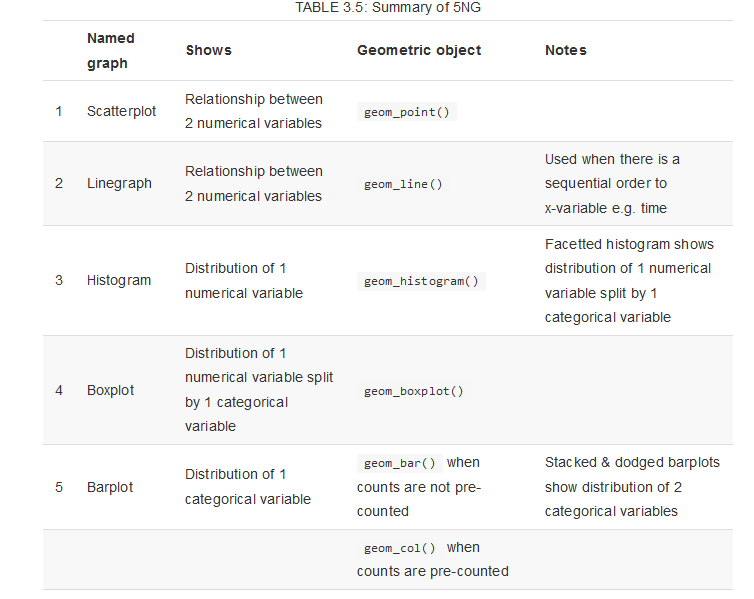
\includegraphics{figures/graph.table.png}

Table 3.5 from Modern Dive
\url{http://moderndive.netlify.com/index.html}

\begin{center}\rule{0.5\linewidth}{0.5pt}\end{center}

\end{document}
